\section{Concept}
%TODO: Paste concept and make it awesome


\subsection{First Idea}


The first idea about this application came to us because our team member Jakub is using an online note taking tool  (in this case apple notes) to keep track of his weekly schedule. Using this note tool to organize the schedule requires more work than necessary. Furthermore it can become a little bit unclear to navigate around the different days and tasks for the week. As we conducted research we were not able to find any application that supports the functionality we would like, meaning an application that has functionality that could be described as some kind of mix between a calendar app and a simple todo list. Our goal is to create an application that lets you plan your task for the next 7 days but not any further. In order to have the schedule available at all times and all devices we decided to create a responsive web application that can run on any device with a modern browser, including desktop computers, smartphones and tablets. User registration and authentication permits for anyone to use this app for his personal schedule planning. The image below shows an example of how our team member Jakub used his note taking app to create his weekly schedule. There is a section for each day of the week as well as another section “stack” for unassigned tasks.   

	\begin{figure}[H] 
		\centering 
		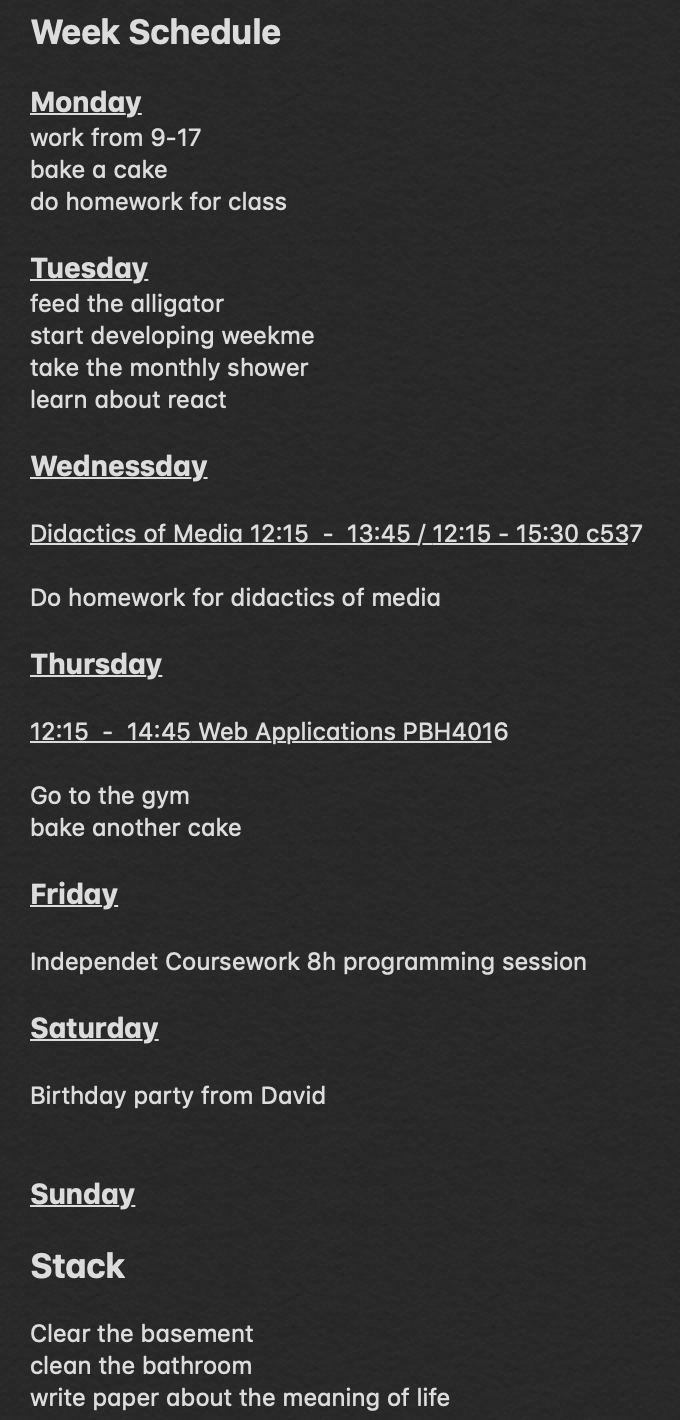
\includegraphics[height=12.2cm]{figures/idea}     
		\caption{Schedule inside Note Taking App}      
	\end{figure}  

\cleardoublepage 

\subsection{First Draft}  
	
The image below demonstrates our first draft of our WeekMe application. The days monday to friday each get their own separate space as well as the stack where unassigned task are collected. Each task is represented by a rectangle. Rectangles can be edited, moved around to another day or to the stack or deleted. For our first prototype we decided to use a framework called Gridstack.js. This framework provides functionality for creating flexible and automatically resizable grids that adapt to its contents. The different task within the grid can be moved around by using drag\&drop. To make sure user always are aware which day of the week we currently have we decided to highlight the current day in a different color. In order to not lose any unfinished tasks we decided to move them back to the stack once their due day has passed. Our top priority was to create a simple and clear user interface and include only the very least functionality that is needed to plan ahead one week and not more.   
 
 	\begin{figure}[H] 
		\centering 
		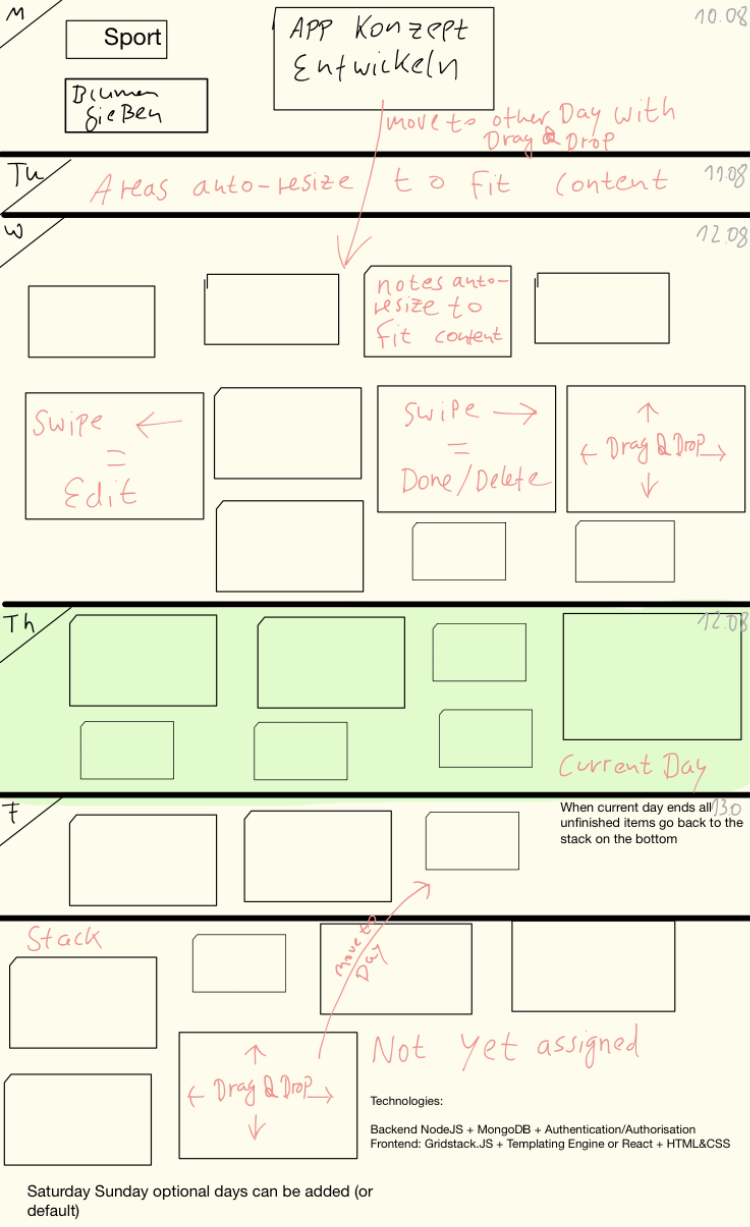
\includegraphics[height=14.2cm]{figures/firstdraft}    
		\caption{First Draft}     
	\end{figure}  

\subsection{Second Draft}

As we found some weaknesses in our first design as well as some technical difficulties that came with the way we had set up our architecture and the technologies we used we decided to use make some big changes to our application. 
We decided to drop Gridstack.js from our project as the tool has some quirks and disadvantages that we had not foreseen previously.  
Moving around task in the grid caused unexpected arrangement problems and sometimes task would disappear entirely from the screen. 
After giving it a reasonable amount of time we decided that the drag and drop functionality of gridstack is not really suited for mobile platforms anyway, 
therefore we switched to using a Bootstrap Grid as the basis for our layout. \\
The second has a design similar to the first draft. 
The weekday are listed vertically and contain the assigned tasks. 
A plus icon in the lower right corner of the screen lets the user create a new task. 
If it is clicked a popup is displayed where the user can enter the text for the new task. 
In the popup the user can also select a colour for the task to help him in categorising or prioritising his tasks or for whatever the user might want to use it for. 
The next step in the creation process is another popup that lets the user select a due-day for his new task or alternatively the stack. \\
To interact with an existing task note the user can just click/tap on it. 
This will highlight the task, select the text and show the editing options. 
Clicking or tapping a second on the same task will deselect it. 
Double clicking/tapping shows an expanded version of the task that will also show the full text for longer descriptions. \\
The edit and delete options will shrink into small icons to give more space to the text. 
Another double click/tap on the task or a single click/tap outside changes it back to its standard size. \\
The available options include “edit” and “delete” on the bottom of the screen which are used to edit or delete tasks. 
On the top of the screen the “stack” and “day” are displayed that can be used to move the task onto the stack or select another day. \\
To move the position of a task within a day, it has to be selected first. Afterwards it can be moved to another tasks position by clicking/tapping on it. 
All tasks that are right to the task will move one position farther to the right (Similar to how you organise your Appicons on the iOS home screen). 
When selecting a task there is also an empty “ghost task” added as last task on that day that allows moving it to its position. \\
If a task on the stack is selected the “stack” option is replaced by a “today” option that moves the task from the stack to the current day. The other options are the same as for all other tasks. \\
In the upper right corner of the screen a burgermenu is located that can collapse to show menu items “settings”, “profile”, “reoccurring tasks” and “logout”. \\
Selecting “reoccurring tasks” gives the user the option to create tasks that will repeat weekly. 
Those tasks will not be onto the stack if they’re past their due-date. 
Furthermore all existing “reoccurring tasks” are listed and can be edited and deleted. 

\subsection{Final Draft}

We modified the second draft a little bit to keep the application more simple and intuitive for the user. \\
In our final draft the task-creation-process can only be started by clicking on a plus (+) symbol in one of the day or stack containers. This gives the user the possibility to create a task in just one step. The user only need to enter a text for the task and click on done. If he wishes he may furthermore change the color or switch the day in case he changed his mind. \\
The adding of a new task and the editing of an existing task will now be processed in the same popup structure so the user can get familiar quickly with the layout and functions. \\
The user can choose between six colours on the colour-picker-popup which is part of the add/edit –popup. We decided to use just six well-chosen colours cause we thought a colour-picker module where you can mix all colours is to overloaded and in some cases more confusing than helpful. The users may use these colours as they wish, for example to prioritise or categorise their tasks. \\
There is no more need for drag and drop in our solution to arrange the tasks. It’s possible to change the position of a task by simply selecting the task with a click and another click on the position you want the task to be. The new position can either be the position of another task or the first free spot inside a day or stack container.  The other tasks will arrange accordingly. The way our task are ordered and arranged was inspired by the way iOS handles their app icons on the home screen. 



